% Options for packages loaded elsewhere
\PassOptionsToPackage{unicode}{hyperref}
\PassOptionsToPackage{hyphens}{url}
\documentclass[
  ignorenonframetext,
]{beamer}
\newif\ifbibliography
\usepackage{pgfpages}
\setbeamertemplate{caption}[numbered]
\setbeamertemplate{caption label separator}{: }
\setbeamercolor{caption name}{fg=normal text.fg}
\beamertemplatenavigationsymbolsempty
% remove section numbering
\setbeamertemplate{part page}{
  \centering
  \begin{beamercolorbox}[sep=16pt,center]{part title}
    \usebeamerfont{part title}\insertpart\par
  \end{beamercolorbox}
}
\setbeamertemplate{section page}{
  \centering
  \begin{beamercolorbox}[sep=12pt,center]{section title}
    \usebeamerfont{section title}\insertsection\par
  \end{beamercolorbox}
}
\setbeamertemplate{subsection page}{
  \centering
  \begin{beamercolorbox}[sep=8pt,center]{subsection title}
    \usebeamerfont{subsection title}\insertsubsection\par
  \end{beamercolorbox}
}
% Prevent slide breaks in the middle of a paragraph
\widowpenalties 1 10000
\raggedbottom
\AtBeginPart{
  \frame{\partpage}
}
\AtBeginSection{
  \ifbibliography
  \else
    \frame{\sectionpage}
  \fi
}
\AtBeginSubsection{
  \frame{\subsectionpage}
}
\usepackage{iftex}
\ifPDFTeX
  \usepackage[T1]{fontenc}
  \usepackage[utf8]{inputenc}
  \usepackage{textcomp} % provide euro and other symbols
\else % if luatex or xetex
  \usepackage{unicode-math} % this also loads fontspec
  \defaultfontfeatures{Scale=MatchLowercase}
  \defaultfontfeatures[\rmfamily]{Ligatures=TeX,Scale=1}
\fi
\usepackage{lmodern}
\ifPDFTeX\else
  % xetex/luatex font selection
\fi
% Use upquote if available, for straight quotes in verbatim environments
\IfFileExists{upquote.sty}{\usepackage{upquote}}{}
\IfFileExists{microtype.sty}{% use microtype if available
  \usepackage[]{microtype}
  \UseMicrotypeSet[protrusion]{basicmath} % disable protrusion for tt fonts
}{}
\makeatletter
\@ifundefined{KOMAClassName}{% if non-KOMA class
  \IfFileExists{parskip.sty}{%
    \usepackage{parskip}
  }{% else
    \setlength{\parindent}{0pt}
    \setlength{\parskip}{6pt plus 2pt minus 1pt}}
}{% if KOMA class
  \KOMAoptions{parskip=half}}
\makeatother
\usepackage{longtable,booktabs,array}
\newcounter{none} % for unnumbered tables
\usepackage{calc} % for calculating minipage widths
\usepackage{caption}
% Make caption package work with longtable
\makeatletter
\def\fnum@table{\tablename~\thetable}
\makeatother
\usepackage{graphicx}
\makeatletter
\newsavebox\pandoc@box
\newcommand*\pandocbounded[1]{% scales image to fit in text height/width
  \sbox\pandoc@box{#1}%
  \Gscale@div\@tempa{\textheight}{\dimexpr\ht\pandoc@box+\dp\pandoc@box\relax}%
  \Gscale@div\@tempb{\linewidth}{\wd\pandoc@box}%
  \ifdim\@tempb\p@<\@tempa\p@\let\@tempa\@tempb\fi% select the smaller of both
  \ifdim\@tempa\p@<\p@\scalebox{\@tempa}{\usebox\pandoc@box}%
  \else\usebox{\pandoc@box}%
  \fi%
}
% Set default figure placement to htbp
\def\fps@figure{htbp}
\makeatother
\setlength{\emergencystretch}{3em} % prevent overfull lines
\providecommand{\tightlist}{%
  \setlength{\itemsep}{0pt}\setlength{\parskip}{0pt}}
% Auto-generated by infrastructure/rendering/_pdf_latex_helpers.py::extract_math_font_preamble.
% Minimal header passed to Pandoc via -H so Beamer slides pick up the same math font
% as the combined-PDF path. Adjust the manuscript's preamble.md to change the font globally.
\usepackage{unicode-math}
\setmathfont{latinmodern-math.otf}

% Slide layout defaults for warning-clean scientific decks.
\usepackage{etoolbox}
\IfFileExists{xurl.sty}{\usepackage{xurl}}{}
\IfFileExists{seqsplit.sty}{\usepackage{seqsplit}}{\newcommand{\seqsplit}[1]{#1}}
\protected\def\breakseq#1{\seqsplit{#1}}
\protected\def\breaktt#1{\begingroup\ttfamily\seqsplit{#1}\endgroup}
\setlength{\emergencystretch}{6em}
\tolerance=5000
\hbadness=10000
\hfuzz=1pt
\setlength{\tabcolsep}{2pt}
\AtBeginEnvironment{longtable}{\tiny\renewcommand{\arraystretch}{0.86}\setlength{\tabcolsep}{1pt}}
\AtBeginEnvironment{tabular}{\tiny\renewcommand{\arraystretch}{0.86}\setlength{\tabcolsep}{1pt}}

% Natbib and cross-reference fallbacks — slides don't load natbib
% or cleveref, but combined-PDF manuscript prose may emit these
% commands. The fallback renders citations as a bracketed key list
% and cross-references as detokenized labels so slides don't fail on
% undefined control sequences or raw underscores. \providecommand is
% a no-op if packages load later.
\providecommand{\citep}[1]{[#1]}
\providecommand{\citet}[1]{#1}
\providecommand{\citealp}[1]{#1}
\providecommand{\citeauthor}[1]{#1}
\providecommand{\citeyear}[1]{#1}
\providecommand{\cref}[1]{\texttt{\detokenize{#1}}}
\providecommand{\Cref}[1]{\texttt{\detokenize{#1}}}
\usepackage{bookmark}
\IfFileExists{xurl.sty}{\usepackage{xurl}}{} % add URL line breaks if available
\urlstyle{same}
% fallback for those not using the hyperref driver hyperxmp:
\makeatletter
\@ifundefined{xmpquote}{\newcommand{\xmpquote}[1]{#1}}{}
\makeatother
\hypersetup{
  hidelinks,
  pdfcreator={LaTeX via pandoc}}

\author{\texorpdfstring{}{}}
\date{}

\begin{document}

\section{Results}\label{sec:results}

\begin{frame}[fragile,allowframebreaks]{Results}
This section presents the exploratory analysis of the shipped dataset.
Every figure and the summary table are produced by the thin analysis
script
(\href{https://github.com/docxology/template/blob/main/projects/templates/template_eda_notebook/scripts/eda_analysis.py}{\breaktt{scripts/eda\_analysis.py}}),
which calls the tested figure-data preparers in
\breaktt{src/eda/figures.py}. Running the script regenerates the figures
under \texttt{output/figures/} and the summary CSV under
\texttt{output/data/}; the prose below describes what those artifacts
show.
\end{frame}

\begin{frame}[fragile,allowframebreaks]{Dataset and missingness}
\protect\phantomsection\label{dataset-and-missingness}
The dataset contains 120 subject records across three groups
(\texttt{alpha}, \texttt{beta}, \texttt{gamma}) with three numeric
features: height (cm), weight (kg), and resting heart rate (bpm). A
small number of cells are blank by design. \texttt{load\_dataset()}
preserves these as \texttt{NaN}; \texttt{clean\_dataset()} then drops
rows missing any numeric feature and reports the count. With the shipped
data, four rows are removed, leaving a complete-case dataset for the
analysis below.
\end{frame}

\begin{frame}[fragile,allowframebreaks]{Distributions}
\protect\phantomsection\label{distributions}
\breakseq{[@fig:height\_histogram]} shows the distribution of height across the
complete-case dataset, binned by \breaktt{histogram\_data()} and plotted
by the analysis script.

\begin{figure}
\centering
\pandocbounded{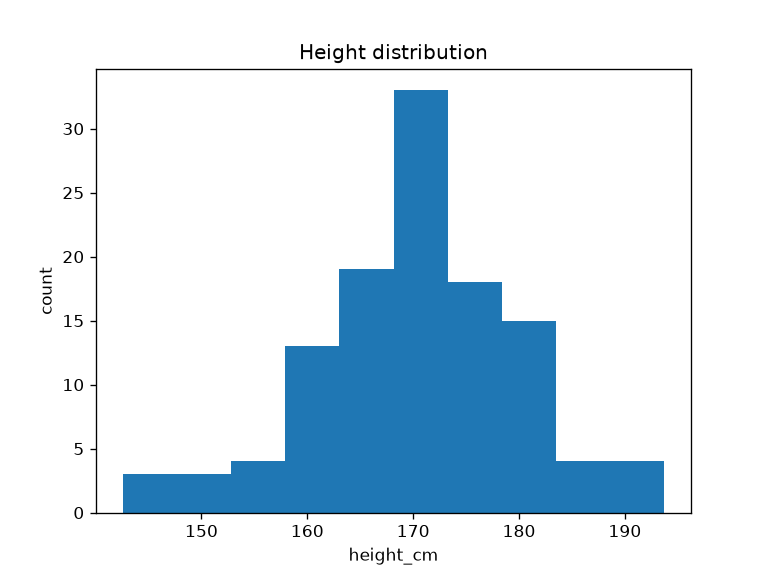
\includegraphics[keepaspectratio,alt={Height distribution: bin counts produced by histogram\_data(frame, "height\_cm", bins=10) in src/eda/figures.py and plotted as a bar chart by scripts/eda\_analysis.py. The bin counts sum to the number of complete-case rows; the shape is the roughly bell-shaped spread expected from the generating process.}]{../figures/height_histogram.png}}
\caption{Height distribution: bin counts produced by
\protect\breaktt{histogram\_data(frame,\ "height\_cm",\ bins=10)} in
\protect\breaktt{src/eda/figures.py} and plotted as a bar chart by
\protect\breaktt{scripts/eda\_analysis.py}. The bin counts sum to the
number of complete-case rows; the shape is the roughly bell-shaped
spread expected from the generating
process.}\label{fig:height_histogram}
\end{figure}
\end{frame}

\begin{frame}[fragile,allowframebreaks]{Group composition}
\protect\phantomsection\label{group-composition}
\breakseq{[@fig:group\_counts]} reports how many complete-case rows fall in
each group, computed by \breaktt{group\_count\_data()} (labels sorted for
deterministic output).

\begin{figure}
\centering
\pandocbounded{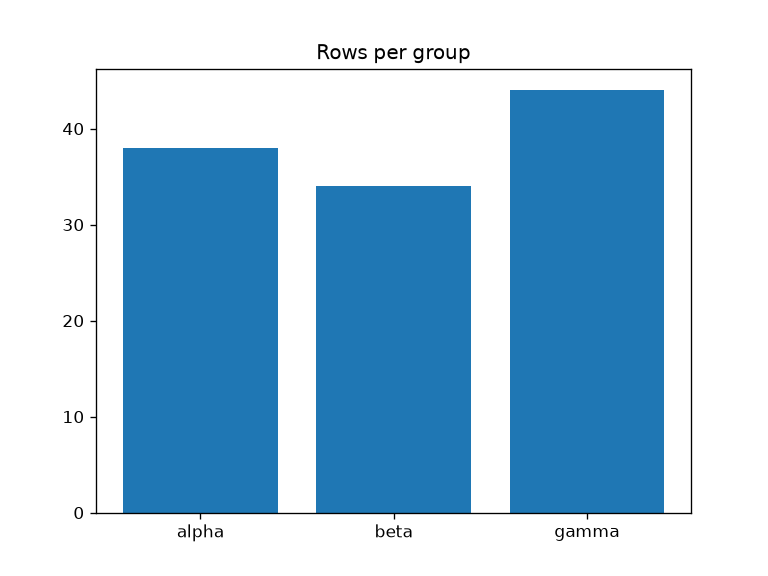
\includegraphics[keepaspectratio,alt={Rows per group: sorted category labels and aligned counts from group\_count\_data(). The three groups are of comparable, though not identical, size; the counts sum to the complete-case row total.}]{../figures/group_counts.png}}
\caption{Rows per group: sorted category labels and aligned counts from
\protect\breaktt{group\_count\_data()}. The three groups are of
comparable, though not identical, size; the counts sum to the
complete-case row total.}\label{fig:group_counts}
\end{figure}
\end{frame}

\begin{frame}[fragile,allowframebreaks]{Correlation structure}
\protect\phantomsection\label{correlation-structure}
\breakseq{[@fig:correlation\_heatmap]} visualizes the Pearson correlation
matrix of the three numeric features, computed by
\breaktt{correlation\_matrix()} and prepared for the heatmap by
\breaktt{correlation\_heatmap\_data()}. The diagonal is unity by
construction and the matrix is symmetric.

\begin{figure}
\centering
\pandocbounded{\includegraphics[keepaspectratio,alt={Feature correlation heatmap: values from correlation\_heatmap\_data() (which wraps correlation\_matrix(method="pearson")) rendered with a diverging colour map on the fixed range {[}-1, 1{]}. Height and weight are strongly positively correlated; resting heart rate is only weakly related to the other two.}]{../figures/correlation_heatmap.png}}
\caption{Feature correlation heatmap: values from
\protect\breaktt{correlation\_heatmap\_data()} (which wraps
\protect\breaktt{correlation\_matrix(method="pearson")}) rendered with a
diverging colour map on the fixed range \([-1, 1]\). Height and weight
are strongly positively correlated; resting heart rate is only weakly
related to the other two.}\label{fig:correlation_heatmap}
\end{figure}

\breaktt{strongest\_pairs(matrix,\ top\_n=3)} ranks the distinct feature
pairs by absolute correlation while preserving sign. On the shipped data
the dominant relationship is \textbf{height \textasciitilde{} weight} (a
strong positive correlation, by design), followed by the comparatively
weak \textbf{height \textasciitilde{} resting heart rate} (slightly
negative) and \textbf{weight \textasciitilde{} resting heart rate}. This
ranking is the single most useful artifact of the first pass: it points
directly at the relationship worth modelling next.
\end{frame}

\begin{frame}[fragile,allowframebreaks]{Summary statistics}
\protect\phantomsection\label{summary-statistics}
The analysis script writes a per-column summary table to
\breaktt{output/data/summary\_statistics.csv} from
\breaktt{summary\_statistics()}. Each row reports the count of
non-missing observations, mean, sample standard deviation, minimum,
median, and maximum for one numeric feature.

\begin{longtable}[]{@{}ll@{}}
\caption{Summary-statistics table written by the analysis script from
\protect\breaktt{src/eda/statistics.py::summary\_statistics()}. The
concrete numbers are reproduced verbatim by running the script --- the
manuscript intentionally does not transcribe volatile values, so prose
and CSV cannot drift.}\label{tbl:summary_statistics}\tabularnewline
\toprule\noalign{}
Column & Reported statistics \\
\midrule\noalign{}
\endfirsthead
\toprule\noalign{}
Column & Reported statistics \\
\midrule\noalign{}
\endhead
\texttt{height\_cm} & count, mean, std, min, median, max \\
\texttt{weight\_kg} & count, mean, std, min, median, max \\
\texttt{resting\_hr\_bpm} & count, mean, std, min, median, max \\
\bottomrule\noalign{}
\end{longtable}

\texttt{group\_means()} complements this with the mean of each numeric
feature within each group; the three group means for height are close
but not equal, reflecting the mild group structure in the generating
process.
\end{frame}

\begin{frame}[fragile,allowframebreaks]{Validation}
\protect\phantomsection\label{validation}
The analysis was validated through the zero-mock \texttt{tests/} suite:

\begin{itemize}
\tightlist
\item
  \textbf{Library tests} assert exact statistics, correlation signs, and
  bin counts against the shipped CSV and hand-built frames.
\item
  \textbf{Script test} runs \texttt{run\_eda()} against a temporary
  output root and confirms real PNG figures and a real summary CSV are
  written.
\item
  \textbf{Notebook test} confirms the walkthrough notebook binds to the
  library's public surface and carries no logic in its cells.
\end{itemize}

All tests pass with coverage exceeding the 90\% project gate, with no
mocks.
\end{frame}

\begin{frame}[allowframebreaks]{Discussion}
\protect\phantomsection\label{discussion}
The results confirm the EDA workflow end to end: missingness is surfaced
and removed with an explicit count, distributions and group composition
are read straight from tested preparers, and the correlation ranking
recovers the designed height--weight relationship. The same functions
back the interactive notebook, the headless script, and this manuscript
--- which is the architectural point of the exemplar. Because every
number is produced by a tested function and regenerated on demand, the
prose here describes structure and provenance rather than transcribing
values that would drift the moment the data changed.
\end{frame}

\end{document}
